\label{ssec:display}
Most people find interacting with robots a very challenging task, especially when they do not deal with them on a regular basis.
It is often difficult for people to hear what the robot is saying and not always intuitive to know when to respond to it. As a solution, we use the integrated screen on the Toyota HSRs' `head' to display useful information. Through the \emph{hero\_ display}\footnote{\url{https://github.com/tue-robotics/hero-display}} we have integrated a few different functionalities. As a default, our Tech United @Home logo with a dynamic background is shown on the screen, as depicted in Figure \ref{fig:hero_display}. When the robot is speaking, the spoken text is displayed, and when it is listening, a spinner along with an image of a microphone is shown. It is also possible to display custom images on this screen.
\begin{figure}[H]
    \centering
	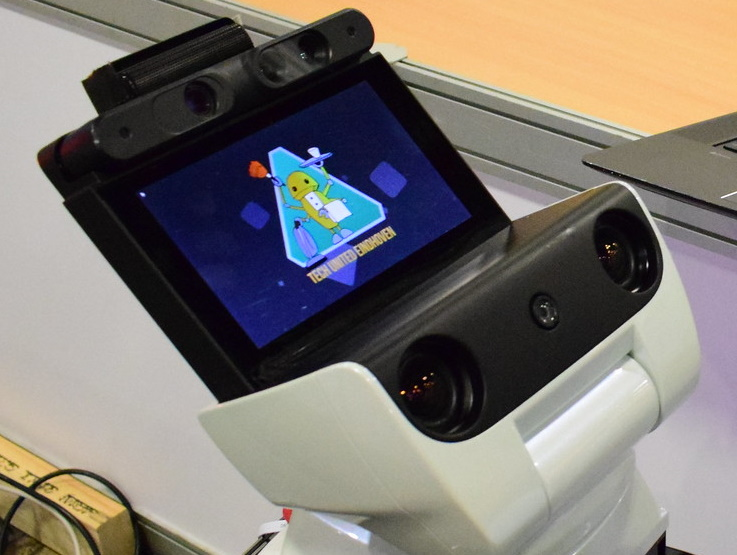
\includegraphics[width=0.45\linewidth]{hero_display_live}
    %\vspace{-0.5em}
	\caption{
		The default status of HERO's head display.}
	\label{fig:hero_display}
\end{figure}